\item Match List I with List II

\def\OptionA{
    \begin{center}
        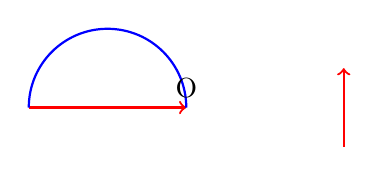
\begin{tikzpicture}
            \draw[thick, red, ->] (0,0) -- (2,0); 
            \draw[thick, blue] (2,0) arc(0:180:1);
            \draw[thick, red, ->] (4,-0.5) -- (4,0.5);
            \node at (2, 0.25) {O};
        \end{tikzpicture}
    \end{center}
}
            
\def\OptionB{
    \begin{center}
        \begin{tikzpicture}
            \draw[thick, red] (0,0) arc(90:-90:0.5);
            \draw[thick, blue, ->] (1,0) -- (2,0);
            \draw[thick, blue] (2,0) -- (4,0);
            \node at (1, 0.75) {O};
        \end{tikzpicture}
    \end{center}
}

\def\OptionC{
    \begin{center}
        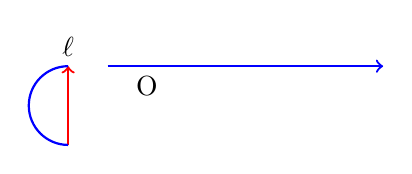
\begin{tikzpicture}
            \draw[thick, red, ->] (0,0) -- (0,1);
            \draw[thick, blue] (0,1) arc(90:270:0.5);
            \draw[thick, blue, ->] (0.5,1) -- (4,1);
            \node at (1, 0.75) {O};
            \node at (0, 1.25) {$\ell$};
        \end{tikzpicture}
    \end{center}
}

\def\OptionD{
    \begin{center}
        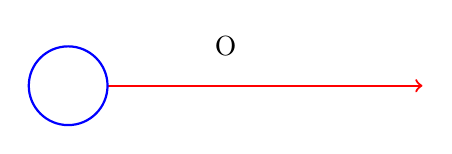
\begin{tikzpicture}
            \draw[thick, red, ->] (0,0) -- (4,0);
            \draw[thick, blue] (0,0) arc(0:360:0.5);
            \node at (1.5, 0.5) {O};
        \end{tikzpicture}
    \end{center}
}

\begin{center}
    \renewcommand{\arraystretch}{2}
    \begin{table}[h]
        \centering
        \begin{tabular}{p{0.25cm}p{8cm}|p{0.25cm}p{5cm}}
        \hline
        & List – I & & List – II \\
        & (Current configuration) & & (Magnitude of Magnetic Field at point O)\\
        \hline
        A.& \OptionA & I.& $B_0 = \frac{\mu_0 I}{4\pi r}[\pi + 2]$\\
        \hline
        B.& \OptionB & II.& $B_0 = \frac{\mu_0 I}{4 r}$\\
        \hline
        C.& \OptionC & III.& $B_0 = \frac{\mu_0 I}{2\pi r}[\pi - 1]$\\
        \hline
        D.& \OptionD & IV.& $B_0 = \frac{\mu_0 I}{4\pi}[\pi + 1]$\\
        \hline
        \end{tabular}
    \end{table}
\end{center}

\begin{tasks}(2)
    \task A $\rightarrow$ III, B $\rightarrow$ IV, C $\rightarrow$ I, D $\rightarrow$ II
    \task A $\rightarrow$ II, B $\rightarrow$ I, C $\rightarrow$ IV, D $\rightarrow$ III
    \task A $\rightarrow$ I, B $\rightarrow$ III, C $\rightarrow$ IV, D $\rightarrow$ II
    \task A $\rightarrow$ III, B $\rightarrow$ I, C $\rightarrow$ IV, D $\rightarrow$ II
\end{tasks}